\documentclass{article}
\usepackage{natbib}
\usepackage[labelfont=bf]{caption}
\usepackage{graphicx}
\bibliographystyle{apalike}
\usepackage{lineno}
\linenumbers

\usepackage{geometry}
\geometry{letterpaper}
\geometry{margin=1in}

\usepackage{setspace}
\doublespacing
\captionsetup[figure]{font={stretch=2}}

\usepackage{authblk}

\newcommand{\matr}[1]{\mathbf{#1}}

\title{Application of the XT3D Multi-Point Flux Approximation to Vertically Staggered Grids \\
	\normalsize or maybe \\
	\LARGE Application of the XT3D Multi-Point Flux Approximation and Enhanced Grid Connectivity to Improve Accuracy of Flows in MODFLOW 6 Models With Steeply Sloping Layers}
\author{
	Xt3d Enthusiast1, Affiliation1  \\
	\and 
	Xt3d Enthusiast2, Affiliation2 \\
	\and 
	Xt3d Enthusiast3, Affiliation3 \\
	\and 
	Xt3d Enthusiast4, Affiliation4 \\
	}

\date{\today}
% Hint: \title{what ever}, \author{who care} and \date{when ever} could stand 
% before or after the \begin{document} command 
% BUT the \maketitle command MUST come AFTER the \begin{document} command! 
\begin{document}

\maketitle

\textbf{Conflict of interest:} None.

\textbf{Key words:} Key words ...

\textbf{Article impact statement:} Article impact statement ...

\begin{abstract}
This is the best paper ever...
\end{abstract}

\section{Introduction}

Some intro stuff here about MODFLOW \citep{modflow6framework, modflow6gwf, modflow6gwt} and XT3D \citep{modflow6xt3d}... Horizontal tops and bottoms of cells... Connection length issue...

Reference and summarize VO results in \cite{bardot2022}. This is an extreme case (virtually impermeable domain surrounding the channel) that nicely accentuates the problem, but there should be some error in any application involving VO grids. Obviously expect it to be a bigger issue for greater offsets. XT3D didn't help, which was initially surprising since it takes into account connection angles and lengths. Not specifying all the angles in the NPF input would cause XT3D to default to "nozee" and therefore assume "horizontal" connections are strictly horizontal, but that was not the case in \cite{bardot2022}.

We explain in this note that it's not just a connection angle and length issue, though that has an effect.  The main problem with a VO grid is insufficient hydraulic communication between grid cells in adjacent layers. (It's not restricted to layered models, but it's convenient to describe it in terms of layers.)  We propose and test a solution to the problem that involves enhanced connectivity between cells.

We present three test models that demonstrate 1) how a VO grid effectively creates wormholes for flow, 2) results on an unmodified VO DIS grid, 3) results on corresponding DISU grid with enhanced connectivity. Results suggest that enhanced connectivity resolves the issue.

%\begin{figure}[ht]
%	\centering
%	\includegraphics[scale=0.6]{figures/fig1.pdf}
%	\caption{This is the first figure.}
%	\label{fig:firstfigure}
%\end{figure}

\section{Theoretical Background}

Explain vertically offset (VO) grids and the connection angle/length issue in more detail than in the Intro. Discuss areas.

Summarize XT3D and how it accounts for connection angle/length.  Reference demonstration by \cite{bardot2022} that, in spite of that, XT3D doesn’t really improve things for a steeply sloping grid.  Must be something else going on in VO grids.

Explain wormholes and how they induce horizontal flow in the sloping channel regardless of XT3D.
\begin{itemize}
	\item Grid with “connector cells”
	\item Role of flows between layers
	\item Shutting off flows between layers using extreme anisotropy in connector cells
	\begin{itemize}
		\item Sloping flow in connector cells
		\item Horizontal flow in flat-top cells
	\end{itemize}
	\item Squashing of connector cells VO grid with horizontal flows and “wormholes”
\end{itemize}

Proposed solution is to introduce cross-connections between layers.

\section{Approach}

Summarize the overall approach here.

Will use a DISV plan-view model with connector cells and XT3D to demonstrate the "wormhole" effect discussed in the Theoretical Background in the limit as connector cells are squashed out. (Also can look at the other limit, as flat-top cells are squashed and connector cells dominate, so grid follows the channel boundary.)

Will use a DIS cross-sectional model to show results you get on a vertically staggered grid (without cross-connections), with and without XT3D. Basically show that we can reproduce what \cite{bardot2022} found.

Will convert the DIS grid to a DISU grid with cross-connections and show improved results, with and without XT3D.

\section{Description of Test Problems}

Describe the test problem setups here.

\subsection{Test problem 1 (DISV plan-view with connector cells)}

Test problem 1...

\begin{figure}
	\begin{center}
	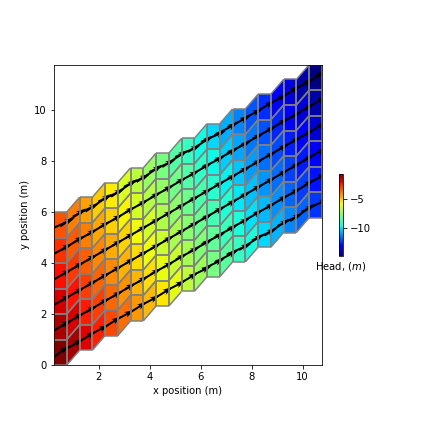
\includegraphics{../figures/worm-zzag-x-i-head.png}
	\caption{Connector cells are conceptually useful.}
	\label{fig:worm-zzag-x-i-head}
	\end{center}
\end{figure}

\begin{figure}
	\begin{center}
	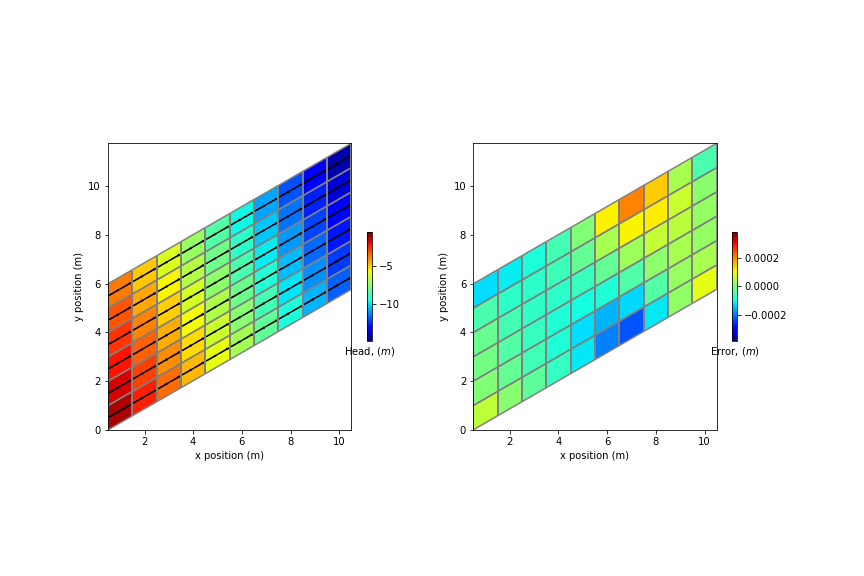
\includegraphics{../figures/worm-smth-x-i-head.png}
	\caption{Smooth is good.}
	\label{fig:worm-smth-x-i-head}
	\end{center}
\end{figure}

\begin{figure}
	\begin{center}
	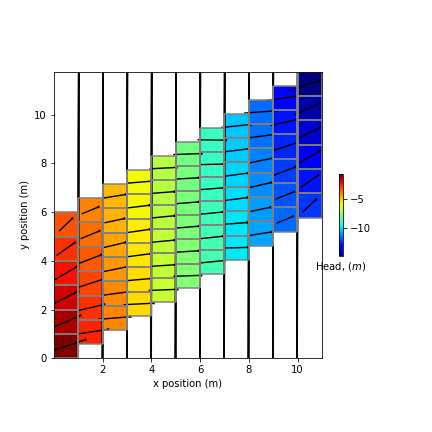
\includegraphics{../figures/worm-sstp-x-a-head.png}
	\caption{Wormholes are bad.}
	\label{fig:worm-sstp-x-a-head}
	\end{center}
\end{figure}

\subsection{Test problem 2 (DIS cross-sectional)}

Test problem 2...

\subsection{Test problem 3 (DISU cross-sectional with cross-connections)}

Test problem 3...

\begin{figure}
	\begin{center}
	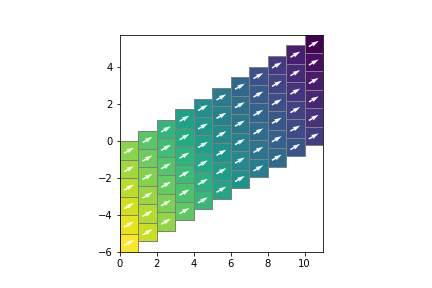
\includegraphics{../figures/mymodel-x-cc-head.png}
	\caption{Cross-connections are good.}
	\label{fig:mymodel-head}
	\end{center}
\end{figure}

\section{Results and Discussion}

\section{Conclusions}

\section{Acknowledgments}
Thank all those reviewers.

\section{Supporting Information}

\section{Appendix}

\bibliography{references.bib}

\end{document}
